\renewcommand{\NomeBloco}{\textit{APS\_digitalized}}
\renewcommand{\NomeBlocoNoUnderline}{apsdigitalized}
\renewcommand{\NomePTab}{tab_\NomeBlocoNoUnderline}
\renewcommand{\NomeSTab}{tab_\NomeBlocoNoUnderline2}
\renewcommand{\NomePFig}{fig_\NomeBlocoNoUnderline}
\renewcommand{\NomeSFig}{fig_\NomeBlocoNoUnderline2}
\renewcommand{\NomeTTab}{tab_\NomeBlocoNoUnderline3}
\renewcommand{\NomeQTab}{tab_\NomeBlocoNoUnderline4}

\section{APS\_digitalized}
\label{sec_apsdigitalized}

O \textit{APS\_digitalized} \'e o circuito respons\'avel por digitalizar o sinal gerado pelo APS descrito na \autoref{section:APS}. O bloco apresenta as definições de sinais de entrada e sa\'ida referidos na \autoref{\NomeSTab}.

\begin{table}[!h]
\caption{Sinais do bloco \NomeBloco}
\label{\NomeSTab}
\centering
\begin{tabular}{ccll}

    \toprule
    Sinal & Tipo    & Descrição & Observação        \\
    \midrule \midrule
    RESET   & Entrada   & Sinal de tensão de RESET no APS & Ativo em nível baixo\\
    \midrule
    ENABLE   & Entrada   & Sinal de tensão de ENABLE no APS & Ativo em nível alto\\
    \midrule
    Vref   & Entrada   & \begin{tabular}[l]{@{}l@{}}Tensão de refer\^encia utilizada pelo\\ \textit{Comparador}\end{tabular} \\
    \midrule
    Ibias   & Entrada   & Corrente de polarização do comparador \\
    \midrule
    AnOut   & Saída   & \begin{tabular}[l]{@{}l@{}}Sinal de tensão anal\'ogica produzido\\ pelo APS\end{tabular} \\
    \midrule
    DigOut   & Saída   & \begin{tabular}[l]{@{}l@{}}Sinal de tensão digital produzido\\ pelo \textit{Comparador}\end{tabular} \\
    \bottomrule
\end{tabular}
\legend{Fonte: Produzido pelo autor}
\end{table}

O circuito projetado para o bloco \'e demonstrado nas figuras \ref{repblocoAPS} e \ref{repblocoAPS2}.

\begin{figure}[!h]
 \centering
    \centering
    \caption{Circuito CMOS projetado para o bloco \NomeBloco com o circuito do APS explicito} 
    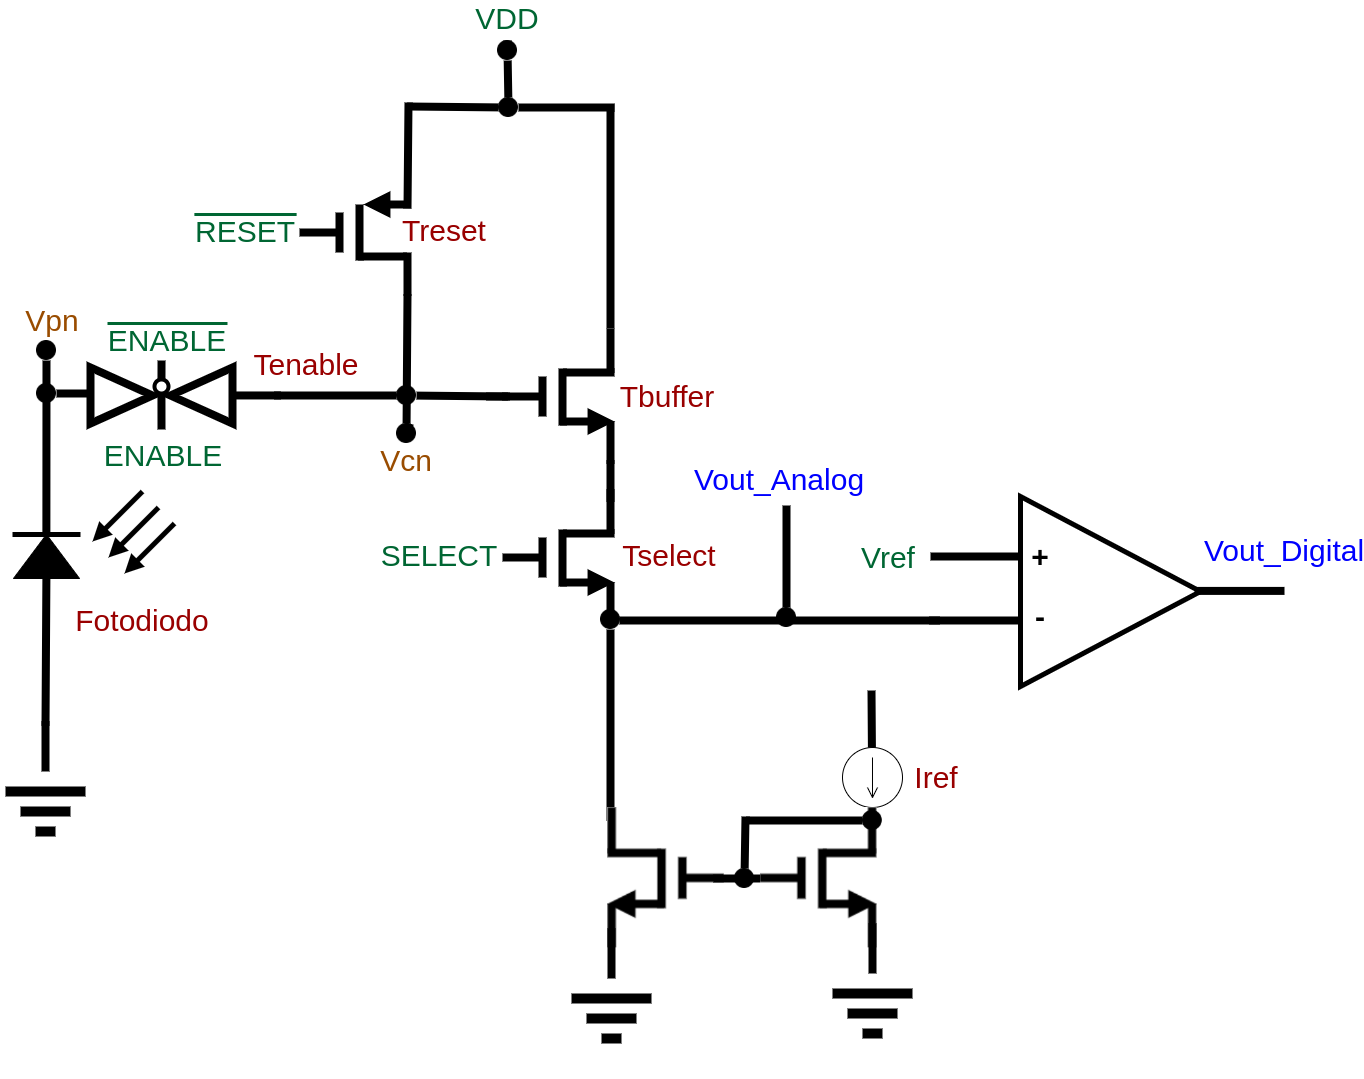
\includegraphics[scale=0.3]{Circuitos/APS_digitalized_rep.png}
    \legend{Fonte: Produzido pelo autor}
    \label{repblocoAPS}
\end{figure}

\begin{figure}[!h]
 \centering
    \centering
    \caption{Circuito CMOS projetado para o bloco \NomeBloco} 
    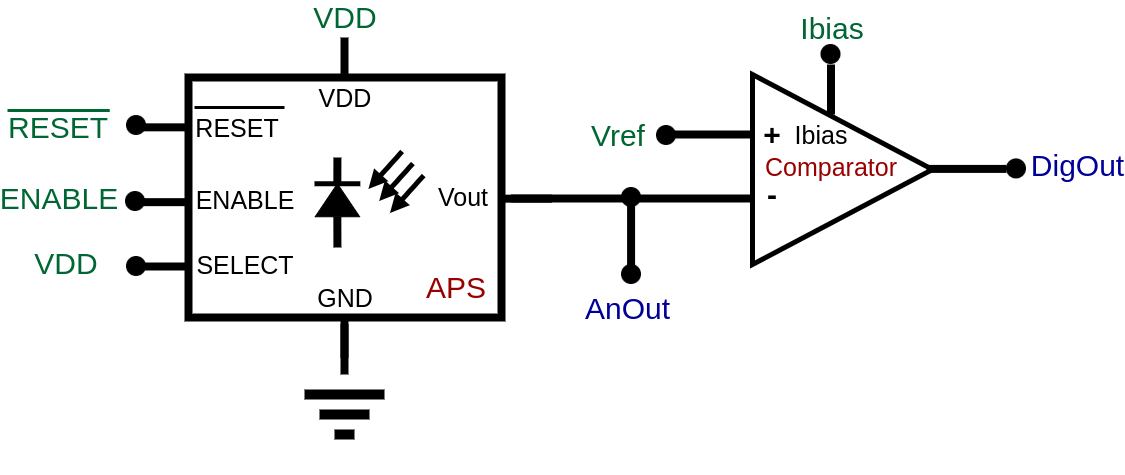
\includegraphics[scale=0.3]{Circuitos/APS_digitalized.png}
    \legend{Fonte: Produzido pelo autor}
    \label{repblocoAPS2}
\end{figure}

\begin{figure}[!h]
 \centering
    \centering
    \caption{\label{\NomeSFig}Representação em bloco do \NomeBloco}
    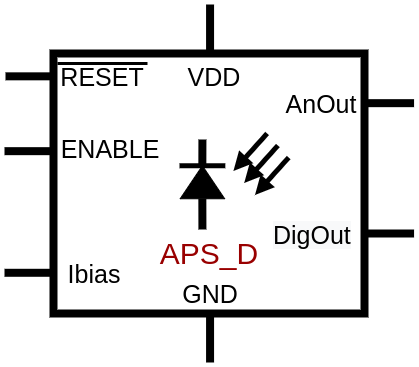
\includegraphics[scale=0.3]{Circuitos/APS_digitalized_block.png}
    \legend{Fonte: Produzido pelo autor}
\end{figure}

A sa\'ida digital do bloco funciona realizando uma comparação entre uma tensão de refer\^encia chamada de \textit{Vref} e a sa\'ida anal\'ogica do APS, chamada de \textit{AnOut}. Quando o valor de \textit{Vref} for maior do que o de \textit{AnOut}, o comparador ir\'a saturar e apresentar um sinal aproximadamente igual a VDD, interpretada como n\'ivel l\'ogico '1'. Quando o valor de \textit{Vref} for menor ou igual do que o de \textit{AnOut}, o comparador ir\'a apresentar um sinal aproximadamente igual a GND em sua sa\'ida, interpretada como n\'ivel l\'ogico '0'.

Utilizando o elemento comparador, podemos ajustar para que a sa\'ida retorne '0' apenas quando for atingido um valor limiar controlado. Como sabemos que a intensidade da corrente fotogerada depende da intensidade da luz captada pelo fotodiodo (\autoref{secao_fotodiodo}), podemos deduzir a informação sobre intensidade luminosa verificando em quanto tempo demora para que se mude de n\'ivel l\'ogico '1' para '0' durante o Est\'agio 2, considerando que o nó $V_{cn}$ apresentava o valor de VDD, que equivale à $AnOut$ apresentar o máximo valor em sua saída (\autoref{eq_voutfinal}). Considerando o atraso no comparador nulo, e desprezando-se as resistências das chaves no bloco APS, podemos utilizar as equações \ref{eq_responsividade}, \ref{eq_modEletFotIl} e \ref{eq_voutfinal} para se obter a \autoref{eq_apsd}.

\begin{equation}
    \label{eq_apsd}
    P_{FD} = \frac{(AnOut_0-V_{ref})(C_{j}+C_{cn})}{R_{\lambda}t_{1-0}}
\end{equation}

Onde:

\begin{itemize}

    \item \textit{P$_{FD}$} \'e a pot\^encia \'optica presente no fotodiodo [\textit{W}]
    \item $AnOut_0$ \'e o valor do nó $AnOut$ no momento que inicia o Período de Integração [$V$]
    \item \textit{$V_{ref}$} \'e a tensão de refer\^encia do comparador [$V$]
    \item \textit{$C_j$} \'e a capacit\^ancia de junção do fotodiodo [\textit{F}]
    \item \textit{$C_{cn}$} \'e a capacit\^ancia do n\'o central do APS [\textit{F}]
    \item $R_{\lambda}$ \'e a responsividade para o comprimento de onda detectado no fotodiodo [$A.W^{-1}$]
    \item $t_{1\_0}$ \'e o tempo do qual o n\'ivel l\'ogico demorou para mudar de '1' para '0', a partir do momento que se inicia o Estágio 2, representado na \autoref{figurataps}, equivalente ao tempo para que a tensão de saída do APS seja igual a Vref [\textit{s}]
    
\end{itemize}

\begin{figure}[!h]
 \centering
    \centering
    \caption{\label{figurataps}Comparação da saída do APS com a tensão de referência do comparador do $APS\_digitalized$ \NomeBloco} 
    \includegraphics[scale=0.3]{Imagens/Graficot.png}
    \legend{Fonte: Produzido pelo autor}
    \label{\NomePFig}
\end{figure}
